\pdfoutput=1
\documentclass[11pt]{article}
\usepackage[review]{EACL2023}
\usepackage{times}
\usepackage{latexsym}
\usepackage[T1]{fontenc}
\usepackage[utf8]{inputenc}
\usepackage{microtype}
\usepackage{inconsolata}
\usepackage{booktabs}
\usepackage{graphicx}
\usepackage{amsmath}
\usepackage{url}
\newcommand{\method}{\textbf{EviRAG}}

\title{\method: Retrieve, Verify, Then Reason for Precision-Critical Scientific QA}

\author{Anonymous EACL submission}

\begin{document}
\maketitle

\begin{abstract}
Large language models can answer scientific questions fluently while still selecting the wrong source, misreading a table, or returning a numerically plausible but unsupported value. We introduce \method, an evidence-first retrieval-augmented generation (RAG) pipeline for questions about the energy, carbon, and water costs of artificial intelligence. The system combines lexical retrieval, dense retrieval, neural reranking, structured generation, citation checks, abstention, and deterministic answer normalization. On the WattBot 2026 Kaggle benchmark, a source-audited candidate reached a public score of 0.966 under the competition's joint answer-and-citation metric. Controlled local experiments show that output repair improves a Qwen3.5-27B development score from 0.6824 to 0.7827, while neural reranking improves Recall@1 on two transfer datasets. On a 41-question WattBot 2025 transfer set, the end-to-end score is 0.731 before normalization and 0.786 after conservative range and unit normalization. On a source-disjoint fold, restricting the final context to three reranked passages improves the score from 0.710 to 0.761; across five grouped folds, LoRA obtains a macro-average of 0.759 (SD 0.162). These results suggest that reliability is not determined by generator scale alone: evidence selection, context size, and structured-output control are separate, measurable capabilities.
\end{abstract}

\section{Introduction}
\label{sec:intro}
Language models are increasingly used to summarize and answer questions about scientific and technical material. In precision-critical settings, however, a fluent answer is not sufficient. The answer must be supported by the correct document, use the correct unit and numerical interpretation, and abstain when the supplied evidence is inadequate. An answer that is almost correct but cites the wrong paper can be as problematic as a conventional hallucination.

Retrieval-augmented generation (RAG) addresses part of this problem by conditioning generation on retrieved documents \citep{lewis2020rag}. Yet a RAG system can still fail in several ways: lexical retrieval can miss a relevant paper, a reranker can order an irrelevant passage above the evidence, a generator can consume its output budget before producing a valid structured answer, and a correct explanation can be paired with an incomplete citation. We therefore treat evidence control as a first-class part of the system rather than as a prompt-only concern.

We investigate the following question:
\begin{quote}
\emph{When scientific QA is evaluated jointly on answer values and citations, how much improvement comes from retrieval quality, neural reranking, structured-output recovery, and deterministic evidence control compared with changing the generator?}
\end{quote}

Our case study is WattBot 2026, a Kaggle benchmark containing questions about the environmental costs of AI and a corpus of scientific papers and reports. The benchmark is useful because it includes direct extraction, numerical calculation, table and figure reading, cross-paper synthesis, and unanswerable questions. We additionally evaluate transfer to WattBot 2025 and to SciFact, a scientific claim-verification dataset \citep{wadden2020scifact}. Our contributions are:
\begin{itemize}
\item an evidence-controlled RAG pipeline combining BM25, dense retrieval, neural reranking, structured generation, and deterministic validation;
\item controlled experiments separating retrieval quality, generator behavior, output validity, citations, and abstention;
\item a cross-year transfer evaluation showing that retrieval transfers strongly while answer normalization remains a bottleneck; and
\item a reproducibility package containing retrieval records, model configurations, output files, validation scripts, and figure-generation code.
\end{itemize}

\section{Background and Related Work}
\label{sec:related}
RAG combines a retriever with a generator so that an answer can be grounded in external evidence \citep{lewis2020rag}. Our lexical baseline uses the probabilistic relevance framework underlying BM25 \citep{robertson2009bm25}. Dense retrieval represents questions and documents in a neural embedding space, which can recover semantically related passages even when the wording differs. A cross-encoder-style reranker then scores a question and candidate passage together, following the general passage-reranking paradigm of \citet{nogueira2019bert}.

Scientific QA has distinctive reliability requirements. QASPER asks information-seeking questions about research papers and provides evidence annotations \citep{dasigi2021qasper}; SciFact asks systems to verify scientific claims against abstracts \citep{wadden2020scifact}. Our task is different in content and scoring, but shares the need to retrieve evidence before answering. Work on hallucination has emphasized that generated text can be unsupported even when it is linguistically coherent \citep{ji2023hallucination}. We operationalize this concern through citation overlap, answer-value matching, abstention, and invalid-output measurements rather than through a new human hallucination annotation scheme.

The scientific domain also motivates the corpus. Prior work measures the energy and carbon cost of model training and deployment \citep{patterson2021carbon,dodge2022carbon,luccioni2024power}, while other work studies water use and inference-energy measurement \citep{li2023thirsty,samsi2023watts,chung2025mlenergy}. These sources provide a realistic mixture of prose, numbers, units, tables, figures, and competing estimates.

\section{Task and Evaluation}
\label{sec:task}
\subsection{WattBot}
Each WattBot question is paired with an answer unit and one or more supporting document identifiers. The system must return an answer value, unit, cited documents, supporting material, and an explanation. The official score weights answer value most heavily, followed by citation overlap and clean abstention. In our local scorer, the overall score is
\begin{equation}
 S = 0.75 V + 0.20 C_{F1} + 0.05 A,
\end{equation}
where $V$ is answer-value correctness, $C_{F1}$ is citation F1, and $A$ measures correct handling of unanswerable questions. Unit matching and explanation validity are additionally checked by the submission validator.

The benchmark contains heterogeneous question types. Direct questions ask for an entity or quoted value. Math questions combine values from multiple documents. Table and figure questions require reading structured or visual evidence. Reconcile questions require reporting multiple values rather than selecting one source. This mixture makes a single model score difficult to interpret without component-level analysis.

\subsection{Transfer Sets}
WattBot 2025 contains 41 labeled questions and a related document collection. SciFact provides scientific claims and evidence-bearing abstracts. We use transfer data only for evaluation and keep its labels separate from the WattBot 2026 test submission.

\section{Evidence-Controlled Pipeline}
\label{sec:method}
Figure~\ref{fig:pipeline} summarizes the system. PDF documents are extracted with page and section information. We then build a hybrid candidate set using BM25 and dense embeddings, fuse the rankings, and apply a neural reranker. The generator sees the question and a compact set of evidence passages, and returns a structured record. Finally, deterministic checks validate citations, answer units, numeric ranges, abstentions, and required fields.

\begin{figure*}[t]
\centering
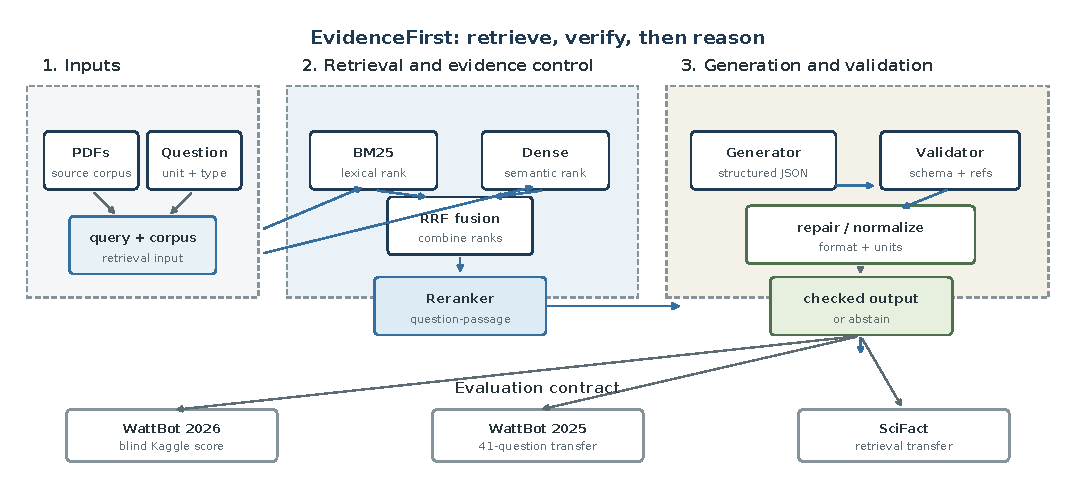
\includegraphics[width=0.98\textwidth]{figures/pipeline.pdf}
\caption{Overview of the evidence-controlled RAG pipeline. The generator is not asked to search the entire corpus; it receives a small, ranked evidence set.}
\label{fig:pipeline}
\end{figure*}

\subsection{Retrieval and Reranking}
For a question $q$, BM25 produces a lexical score for each document or passage. Dense retrieval produces a semantic score using neural embeddings. We combine the ranked lists with reciprocal-rank fusion, retaining candidate passages from both views. A neural reranker then scores each question--passage pair and orders the final evidence list. The reranker is particularly important for questions whose wording differs from the source wording.

\subsection{Structured Generation and Evidence Control}
The generator is prompted to return a fixed schema containing an answer value, unit, reference identifiers, supporting material, and an explanation. A parser rejects malformed outputs. A direct-response repair path is used when a reasoning-mode output reaches its token limit before producing the schema. Citations are constrained to retrieved documents; unsupported identifiers are discarded rather than silently added.

\subsection{Deterministic Normalization}
Some errors are representational rather than semantic. For example, a model may output ``80--90'' when the scorer requires ``[80,90]'', or may report ``10--50 responses per bottle'' when the question asks for bottles per response. Our normalization layer applies only transformations determined by the question unit and explicit answer format. It does not use gold labels and does not replace a substantive model answer with a manually selected value.

\paragraph{Naming convention.} \method{} is the complete method: hybrid lexical--dense retrieval, neural reranking, a compact evidence budget, structured generation, and deterministic validation. BM25, hybrid retrieval, and alternative evidence budgets are ablations of the same method. The preferred configuration identified here is \method-Top3.

\section{Experimental Setup}
\label{sec:setup}
The main WattBot development experiments use the frozen retrieved evidence and a Qwen3.5-27B generator from the Qwen family \citep{qwen3,qwen3embedding}. We compare thinking mode, direct generation, structured-output repair, and conservative field recovery. Additional controlled experiments use a Qwen3.6 mixture-of-experts generator and Kimi K3.1 Pro \citep{kimiwa} on the same 49-question fold. The latter comparisons are diagnostic and are not treated as interchangeable with the full development set.

All retrieval outputs, raw generations, normalized predictions, and scores are saved. The primary public Kaggle score is reported separately from the local experiments because the Kaggle test set is blind. The current source-audited candidate is `testing38\_q157\_q306\_reverted.csv`, which obtained a public score of 0.966. We omit team identity and leaderboard rank in this anonymous version.

\section{Results}
\label{sec:results}
\subsection{Retrieval Transfer}
Table~\ref{tab:retrieval} reports Recall@1 on the two transfer datasets. Reranking improves early recall on both datasets. The hybrid score is not always higher than BM25 at rank one, which is a useful reminder that fusion and reranking should be evaluated together rather than assumed to help every cutoff. QASPER is used only as a retrieval-only diagnostic here; we do not claim an end-to-end WattBot answer score on its full-paper questions.

\begin{table}[t]
\centering
\scriptsize
\begin{tabular}{lrrr}
\toprule
Dataset & BM25 & Hybrid & + reranker \\
\midrule
WattBot 2025 & 75.61 & 66.67 & \textbf{80.77} \\
SciFact & 70.20 & 68.28 & \textbf{82.77} \\
\bottomrule
\end{tabular}
\caption{Retrieval Recall@1 (percent) on transfer datasets. The reranker uses the same candidate set produced by the preceding retrieval stage.}
\label{tab:retrieval}
\end{table}

\begin{figure}[t]
\centering
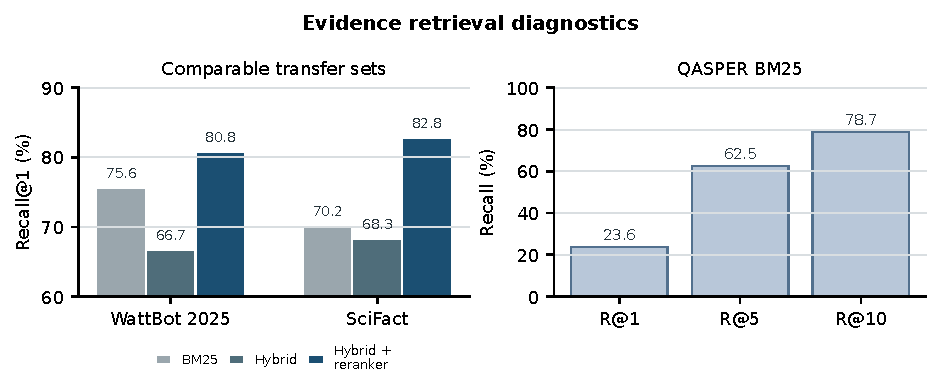
\includegraphics[width=\columnwidth]{figures/retrieval_r1.pdf}
\caption{Recall@1 for the transfer retrieval experiments.}
\label{fig:retrieval}
\end{figure}

\subsection{Generator Reliability}
Table~\ref{tab:generator} shows the most important development result. Always-on reasoning obtains 0.6824. Direct repair raises the score to 0.7827, and conservative recovery raises it slightly further to 0.7831. The improvement is mainly an output-reliability improvement: long reasoning sometimes consumes the output budget before the final JSON record is emitted.

\begin{table}[t]
\centering
\scriptsize
\begin{tabular}{lrrrr}
\toprule
System & $V$ & $C_{F1}$ & $A$ & Overall \\
\midrule
Qwen3.5 thinking & .665 & .667 & 1.000 & .6824 \\
+ direct repair & .767 & .787 & .996 & .7827 \\
+ conservative recovery & .767 & .789 & .996 & \textbf{.7831} \\
Qwen3.6 direct & .718 & .781 & 1.000 & .7450 \\
\bottomrule
\end{tabular}
\caption{Development-set results. $V$ is answer-value matching; $C_{F1}$ is citation F1; $A$ is abstention agreement.}
\label{tab:generator}
\end{table}

\subsection{Unseen-Source and Evidence-Budget Generalization}
To test source transfer, we keep citation-connected source groups within folds. The five grouped source-disjoint LoRA scores are 0.835, 0.793, 0.473, 0.827, and 0.869, giving a macro-average of 0.759 (SD 0.162; range 0.473--0.869). On the same 75-question held-out fold, we also compare retrieval conditions with a fixed Qwen3.5-27B generator. BM25 scores .580, hybrid retrieval .709, reranked top-12 .710, reranked top-6 .687, and reranked top-3 .761. Thus, combining lexical and semantic retrieval is important, but passing every retrieved passage to the generator is not: a compact top-three evidence budget performs best in this evaluation.

\begin{table}[t]
\centering
\small
\begin{tabular}{lrr}
\toprule
Evidence config. & $n$ & Overall \\
\midrule
BM25-only ablation & 75 & .580 \\
Hybrid-retrieval ablation & 75 & .709 \\
Full reranker, top-12 & 75 & .710 \\
Full reranker, top-6 & 75 & .687 \\
\method-Top3 & 75 & $\mathbf{.761}$ \\
\bottomrule
\end{tabular}
\caption{\method{} retrieval and evidence-budget ablations on the same source-disjoint fold.}
\label{tab:evidence-budget}
\end{table}

\subsection{Cross-Year Generalization}
The WattBot 2025 transfer experiment provides a compact test of whether the pipeline depends on the 2026 question wording. The original end-to-end score is 0.731. Applying only the deterministic normalizer raises it to 0.786, a gain of 0.055. Citation F1 is 0.843 and unanswerable-question agreement is 1.000. The result is not evidence that all scientific QA transfers without adaptation: the remaining errors are concentrated in numerical interpretation, cross-paper reasoning, and missing or extra citations.

\begin{figure}[t]
\centering
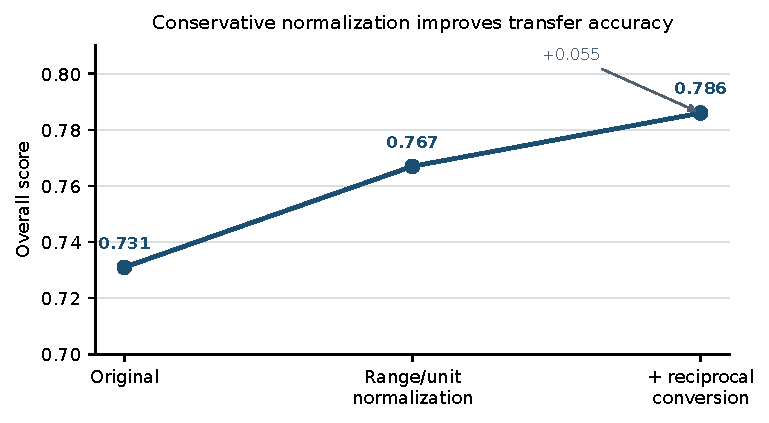
\includegraphics[width=\columnwidth]{figures/normalization.pdf}
\caption{WattBot 2025 score before and after conservative answer normalization.}
\label{fig:normalization}
\end{figure}

\begin{table}[t]
\centering
\scriptsize
\begin{tabular}{lrrr}
\toprule
Transfer condition & Value & Citation F1 & Overall \\
\midrule
Original generation & .683 & .843 & .731 \\
Range/unit normalization & .732 & .843 & .767 \\
+ reciprocal conversion & .756 & .843 & \textbf{.786} \\
\bottomrule
\end{tabular}
\caption{WattBot 2025 transfer results on 41 labeled questions.}
\label{tab:transfer}
\end{table}

\subsection{Blind Kaggle Result}
The best WattBot 2026 candidate obtained a public Kaggle score of \textbf{0.966}. This result is useful as an external benchmark because the test answers are hidden, but it is not used to tune the transfer experiments. The public score should be accompanied by the public/private split and the date of the score in any non-anonymous report because the leaderboard can change.

\section{Analysis}
\label{sec:analysis}
The experiments support four conclusions. First, retrieval and generation are separable. Hybrid retrieval is substantially stronger than BM25 alone, while neural reranking adds little when twelve passages are passed unchanged to the generator. Second, context control matters: the top-three evidence budget outperforms both six and twelve passages. Third, output control is a substantial part of practical QA quality. Fourth, transfer exposes failure modes that a single leaderboard score hides: the five-fold source-disjoint results vary widely, and the WattBot 2025 normalizer recovers formatting and unit errors but cannot solve substantive numerical or cross-paper errors.

These findings are relevant to hallucination and confabulation research. We do not claim to detect every hallucination, and we do not introduce a new human hallucination label set. Instead, we define a narrower operational target: an answer is unreliable when its value is wrong, its citation does not support the value, or it should have abstained. This target is measurable from the benchmark contract and can be reproduced without subjective post-hoc judgments.

\section{Limitations}
\label{sec:limitations}
The evaluation is primarily English and focuses on scientific questions about AI infrastructure and environmental impact. WattBot 2025 is small, with 41 labeled questions, so its transfer score should be interpreted as a stress test rather than a population estimate. SciFact measures scientific claim verification rather than the full WattBot answer schema. The public Kaggle score is a blind benchmark result and does not by itself identify which component caused each gain. Although five grouped source-disjoint folds are reported, the variance is large and the LoRA evaluation uses one seed. The evidence-budget comparison uses one held-out fold and should not be treated as a universal optimum for every corpus. Finally, the system requires substantial GPU resources for dense retrieval, reranking, and long-context generation; reducing this cost is an important follow-up.

\section{Conclusion}
\label{sec:conclusion}
We presented an evidence-controlled RAG pipeline for precision-critical scientific QA. The pipeline combines lexical and neural retrieval, neural reranking, structured generation, citation validation, abstention, deterministic normalization, and an explicit evidence budget. It achieved a public WattBot 2026 score of 0.966, transferred to WattBot 2025 with an end-to-end score of 0.786 after conservative normalization, and reached 0.761 on the source-disjoint top-three evidence condition. The central lesson is simple: improving reliability is not only a matter of selecting a larger generator. Retrieving the right evidence, limiting irrelevant context, preserving a valid output structure, and checking units and citations are separate engineering and research problems.

The submitted code should include the saved retrieval files, model configuration, normalization script, validator, and instructions for running the local evaluation without private API credentials.

\section*{Ethics Statement}
The system is designed to make scientific answers more inspectable, not to replace expert judgment. Environmental estimates in the source literature can be uncertain or incomparable across hardware, geography, and system boundaries. We therefore preserve source identifiers and explanations, report abstention behavior, and avoid presenting a generated answer as an authoritative measurement. External API credentials are kept out of the repository and cached outputs are used for reproducibility when an API is unavailable.

\section*{Acknowledgements}
We thank the WattBot organizers and the authors of the cited scientific datasets and source papers. Computation used local GPUs and the Panther cluster. The authors are responsible for all remaining errors.

\bibliographystyle{acl_natbib}
\bibliography{custom}

\end{document}
